\documentclass[t]{beamer}

\usetheme{simpleucas}


\titlegraphic{
\begin{tikzpicture}[overlay, remember picture]
    \node[anchor=south]  at (current page.south) {
          
\includegraphics[width=\textwidth]{
         ./images/dasfaa.jpg
       }
   };
\end{tikzpicture}
}

\author{
Junjie Huang$^{1,2}$
, Qi Cao$^{1}$
, Ruobing Xie$^{3}$
, Shaoliang Zhang$^{3}$
, Feng Xia$^{3}$
, Huawei Shen$^{1,2}$
, Xueqi Cheng$^{1,4}$
}
\institute{
$^{1}$Data Intelligence System Research Center, \\
Institute of Computing Technology, Chinese Academy of Sciences, Beijing, China
$^{2}$University of Chinese Academy of Sciences, Beijing, China \\
$^{3}$WeChat, Tencent, Beijing, China\\
$^{4}$CAS Key Laboratory of Network Data Science and Technology,\\
Institute of Computing Technology, Chinese Academy of Sciences, Beijing, China \\
\{huangjunjie17s, caoqi, shenhuawei, cxq\}@ict.ac.cn,\\
\{ruobingxie, modriczhang, xiafengxia\}@tencent.com}

\date{\today}

\title{Adversarial Learning Data Augmentation for Graph Contrastive Learning in Recommendation}

\begin{document}


\titlepage

\section{Introduction}

\begin{frame}{Introduction}
    \begin{figure}
        \centering
        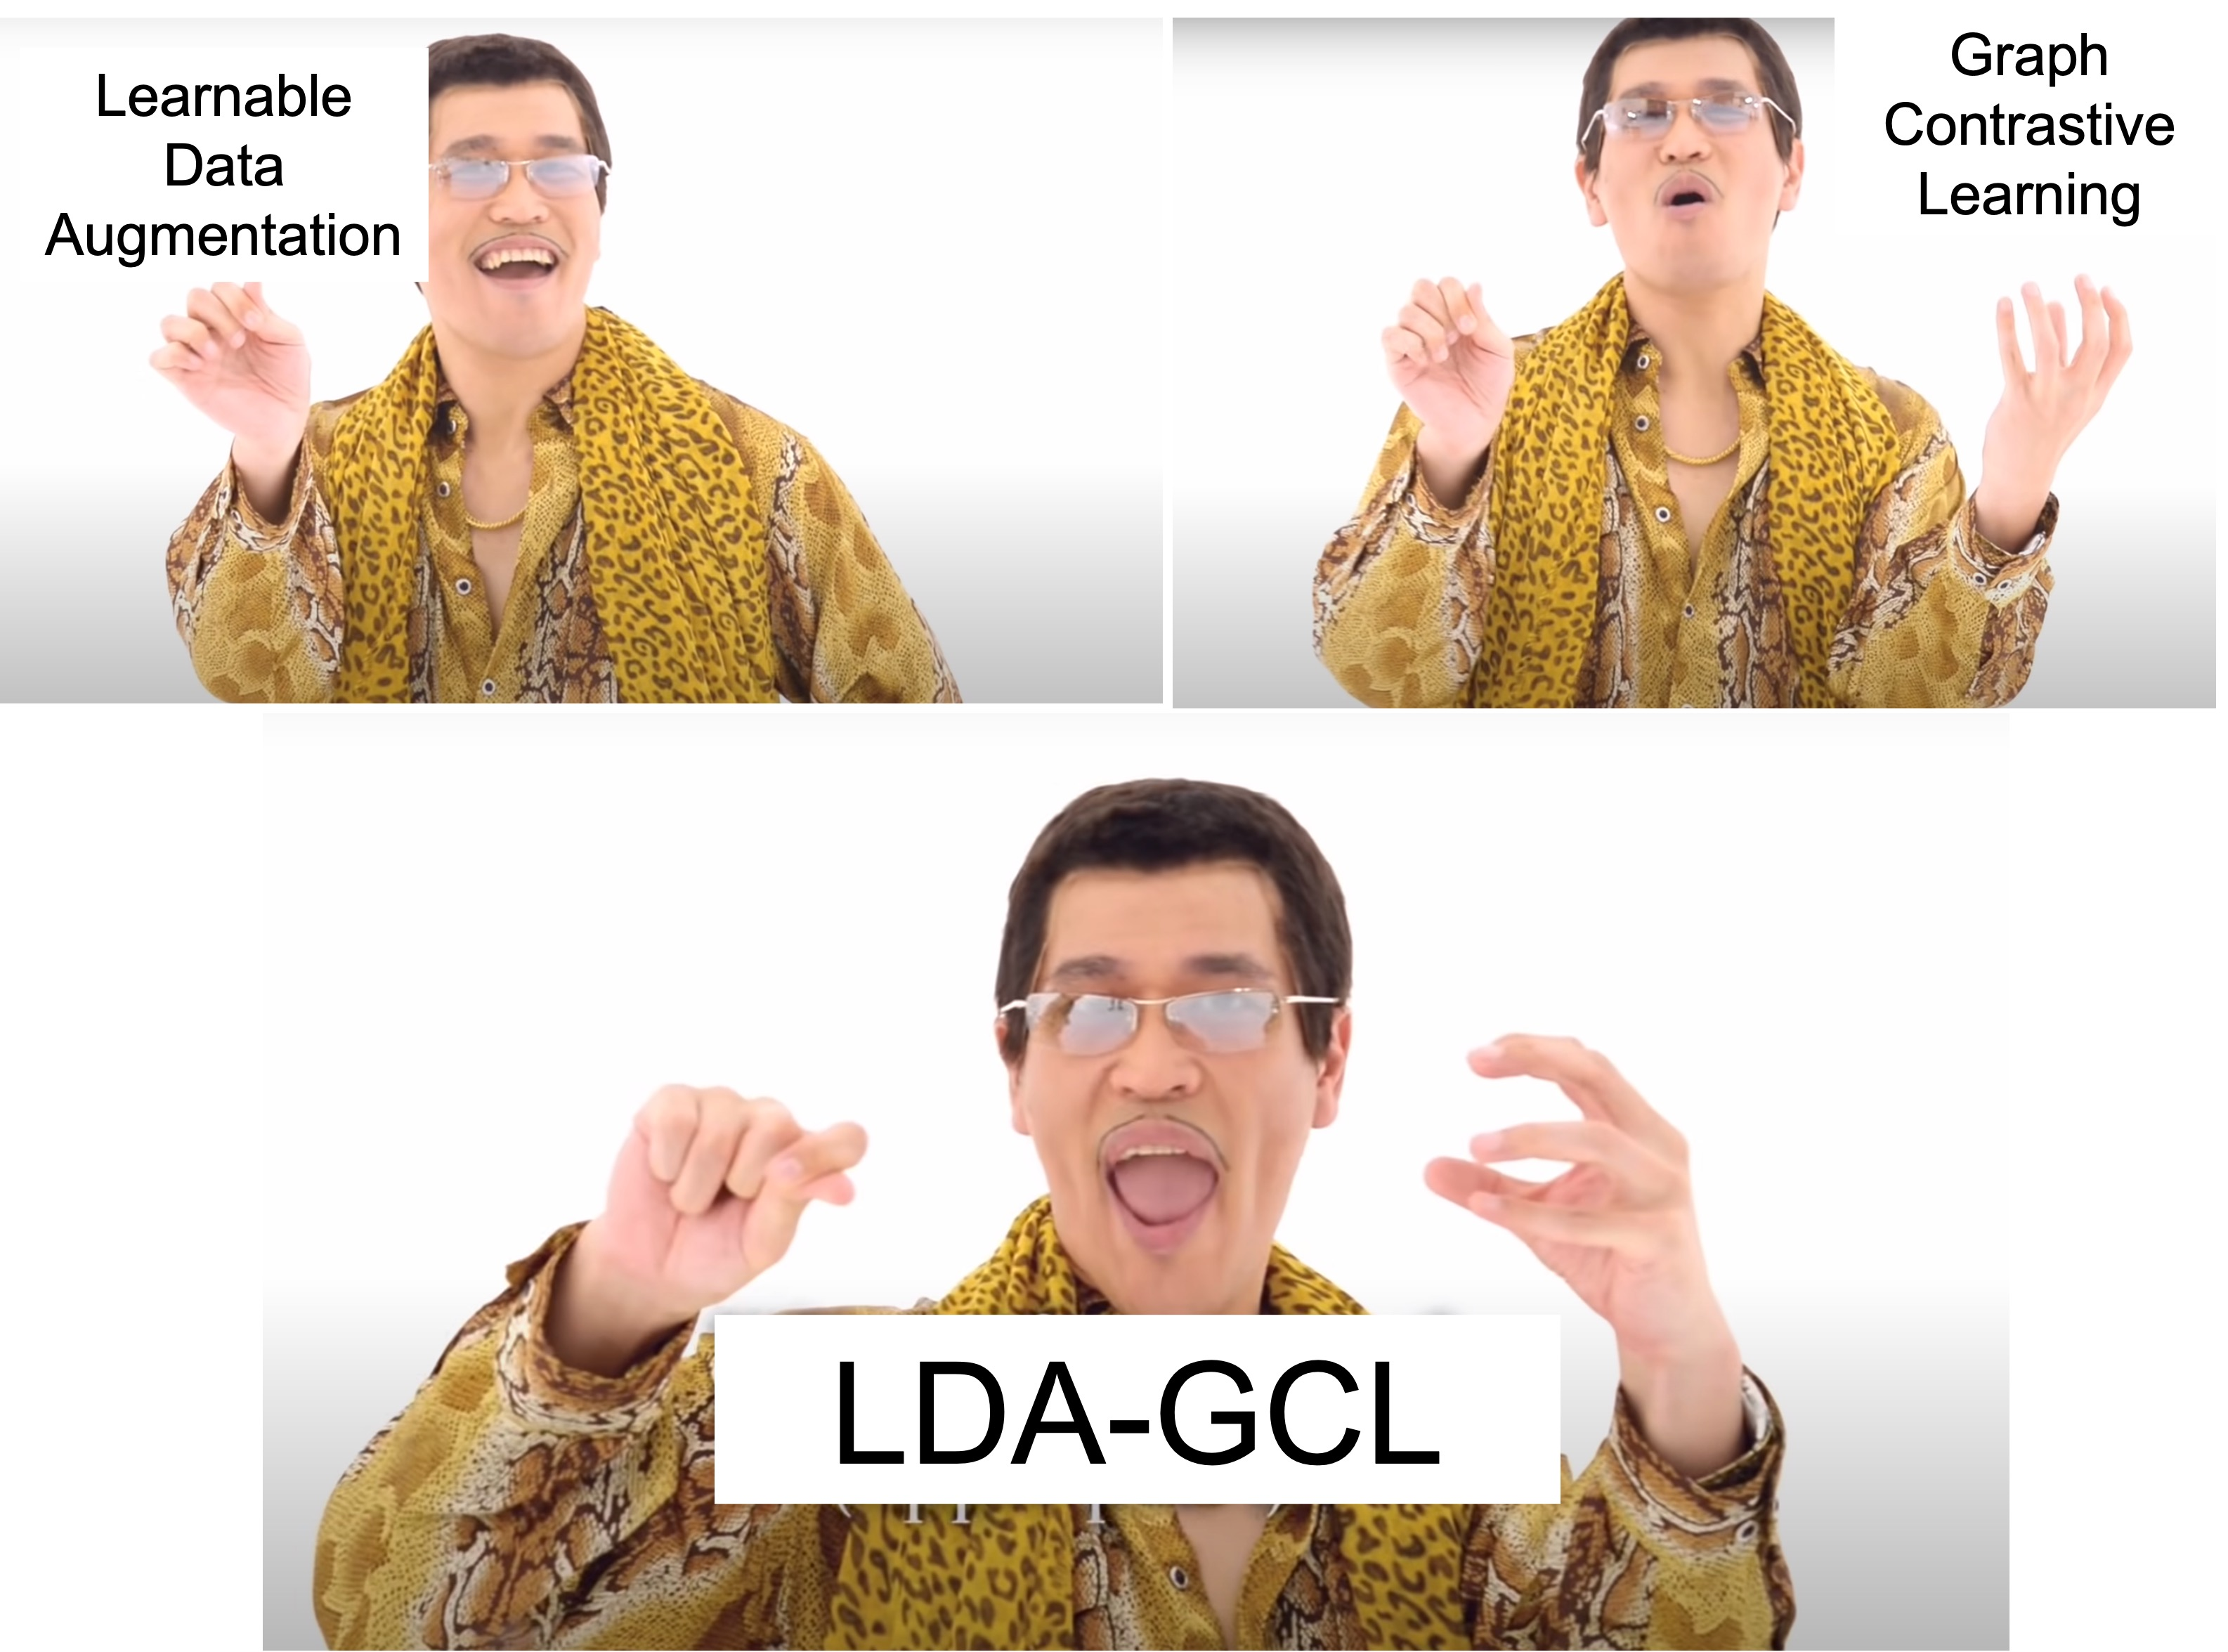
\includegraphics[width=\textwidth]{images/LDA_GCL.jpg}
    \end{figure}
\end{frame}

\begin{frame}{Related Work}
\begin{itemize}
    \item GNN-based  Recommendation
    \begin{itemize}
        \item Matrix Factorization (MF) methods: BPRMF~\tinycite[2012]{rendle2012bpr}, DMF\tinycite[IJCAI2017]{xue2017deep}, NeuMF\tinycite[WWW2017]{he2017neural} 
        \item Auto-encoder (AE) methods: Mult-VAE\tinycite[WWW2018]{liang2018variational}
        \item Graph Neural Networks (GNNs): NGCF~\tinycite[SIGIR2019]{wang2019neural}, LightGCN~\tinycite[SIGIR2020]{he2020lightgcn}, DGCF~\tinycite[WWW2020]{wang2020disentangled}
        \item Most GNN methods in recommender system follow the message-passing scheme~\tinycite[ICML2017]{gilmer2017neural} to utilize the bipartite graph structure.
    \end{itemize}
    \item Contrastive Learning in Recommendation
    \begin{itemize}
        \item Contrastive Learning (CL) as a self-supervised manner, has been applied in Recommender Systems (RS), including SSL+DNN~\tinycite[CIKM2021]{yao2021self}, SGL~\tinycite[SIGIR2021]{wu2021self-sigir}, SimGCL~\tinycite[SIGIR2022]{yu2021self}, NCL~\tinycite[WWW2022]{lin2022improving}.
        \item Graph Contrastive Learning (GCL) is often used to alleviate the \textbf{data sparsity}  and \textbf{popularity bias} problem.
    \end{itemize}
\end{itemize}
    
\end{frame}


\section{Preliminary}
\label{sec:preliminary}

\begin{frame}[allowframebreaks]{GNN-based CF}
\setlistsep{1ex}{0ex}{0ex}
\begin{itemize}
    \item Bipartite Graph in Recommendation
    \begin{itemize}
        \item  As the fundamental recommender system, collaborative filtering (CF) can be modelled as a user-item bipratite graph as $G = (\mathcal{U}, \mathcal{I}, \mathcal{E})$, where $\mathcal{U}$ is the user set, $\mathcal{I}$ is the item set and $\mathcal{E} \subseteq \mathcal{U} \times \mathcal{I}$ is the  inter-set edges. 
        \item $\mathcal{E}$ can be denoted as the user-item interaction matrix $\mathbf{R}\in \{0, 1\}^{|\mathcal{U}| \times |\mathcal{I}|}$.
The adjacency matrix
$
\mathbf{A}=\left[\begin{array}{cc}
\mathbf{0} & \mathbf{R} \\
\mathbf{R}^{\top} & \mathbf{0}
\end{array}\right]
$
is also widely used in~\cite{he2020lightgcn}.

    \end{itemize}

   \item GNN-based Collaborative Filtering
   \begin{itemize}
       \item Based on the bipartite graph $\mathbf{A}$, the general GNN-based CF methods follow the message-passing scheme:
\begin{equation*}
z_{w}^{l} =f_{\text {aggregate }}\left(\left\{z_{v}^{l-1} \mid v \in \mathcal{N}_{w} \cup\{w\}\right\}\right), 
z_{w} =f_{\text {update }}\left(\left[z_{w}^{0}, z_{w}^{1}, \ldots, z_{w}^{L}\right]\right),
\end{equation*}
where $\mathcal{N}$ denotes the neighbor set of node $w$ and $L$ denotes the number of GNN layers. 
    \end{itemize}
\framebreak
    \item LightGCN
    \begin{figure}
        \centering
        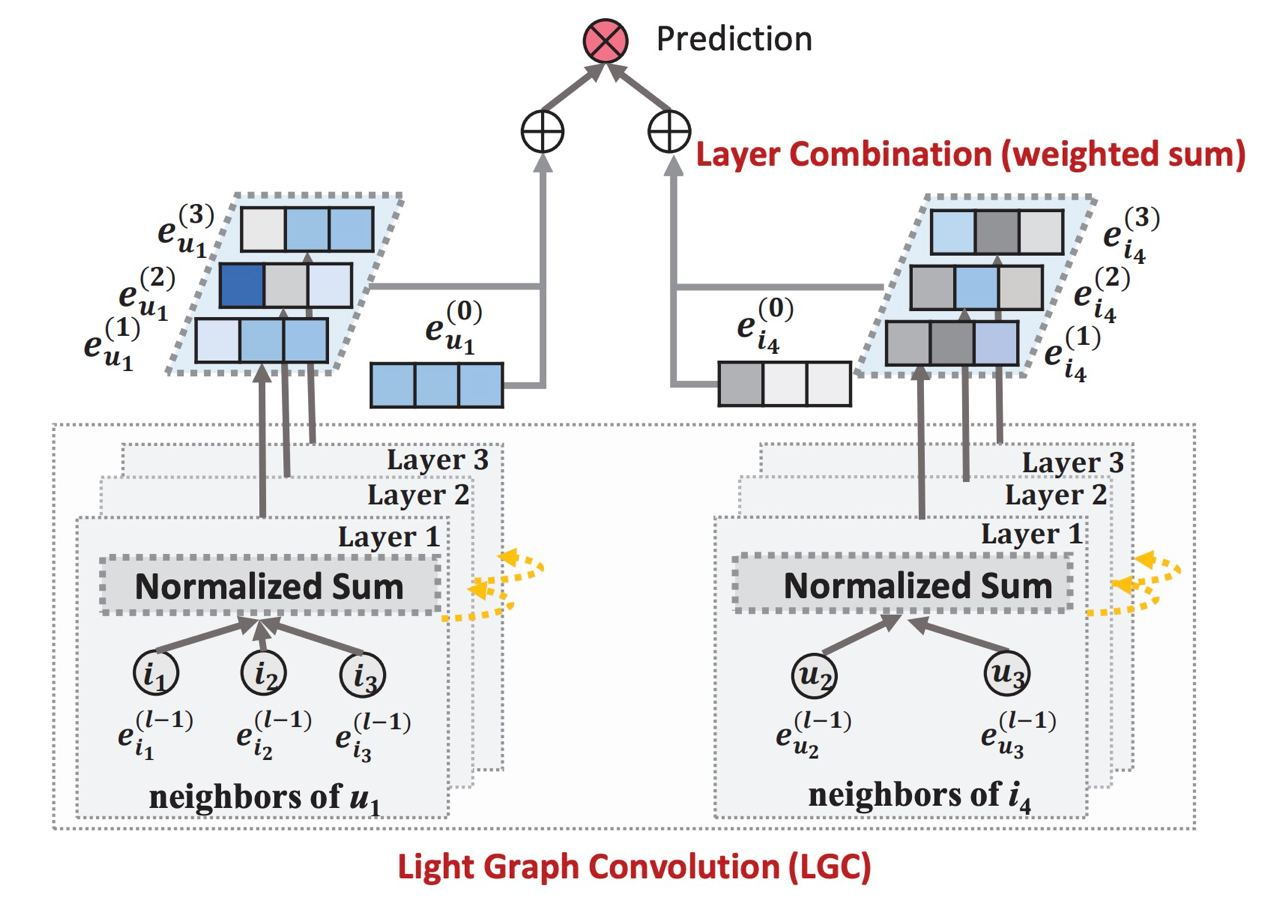
\includegraphics[width=0.4\textwidth]{images/lightgcn.jpg}
        \label{fig:my_label}
    \end{figure}

    
    \begin{itemize}
        \item LightGCN\tinycite[SIGIR2020]{he2020lightgcn} applies a simple weighted sum aggregator:
\begin{equation*}
    \label{eq:lightgcn}
    Z^{l+1} =\left(\mathbf{D}^{-\frac{1}{2}} \mathbf{A} \mathbf{D}^{-\frac{1}{2}}\right) Z^{l}, 
    Z = \frac{1}{L+1}(Z^0 + Z^1 + \cdots + Z^L),
\end{equation*}
where $\mathbf{D}_{ii}=\sum_j \mathbf{A}_{ij}$ is the diagonal matrix and $Z^0$ is initial trainable embeddings.
    \end{itemize}
\framebreak
    \item Loss Function
    \begin{itemize}
        \item Most GNN-based CF methods (e.g., NGCF~\tinycite[SIGIR2019]{wang2019neural}, DGCF~\tinycite[WWW2020]{wang2020disentangled}, and LightGCN~\tinycite[SIGIR2020]{he2020lightgcn}) use the pairwise Bayesian Personalized Ranking (BPR) loss function for the model training:
\begin{equation*}
\mathcal{L}_{\text{BPR}}=\sum_{(u, i, j) \in \mathcal{O}}-\log \sigma\left(\hat{y}_{u i}-\hat{y}_{u j}\right),
\end{equation*}
where $\mathcal{O} = \{(u, i, j) | (u, i)\in \mathcal{O}^+, (u, j)\in \mathcal{O}^-\}$, $\mathcal{O}^+$ and $\mathcal{O}^-$ are the observed and unobserved interactions, respectively.
    \end{itemize}
\end{itemize}
\end{frame}

\begin{frame}[allowframebreaks]{GCL in Recommendation}
\setlistsep{1ex}{0ex}{0ex}
\begin{itemize}
    \item Graph Contrastive Learning in Recommendation
    \begin{itemize}
        \item Data Augmentation
        \begin{itemize}
            \item Common data augmentation is the perturbation of the graph structure due to the absence of node features.(e.g.,  Edge-dropping \tinycite[SIGIR2021]{wu2021self-sigir}.)
            \item \textbf{InfoMin} principle that the good set of views shares the \textit{minimal} information necessary to perform well at the downstream task.
        \end{itemize}
    \end{itemize}

\begin{tikzpicture}[remember picture,overlay]
    \node[anchor=center] (a) at ($(current page.center) + (0.0\textwidth, -0.12\linewidth)$)
    {   
        \resizebox{0.8\textwidth}{!}{
        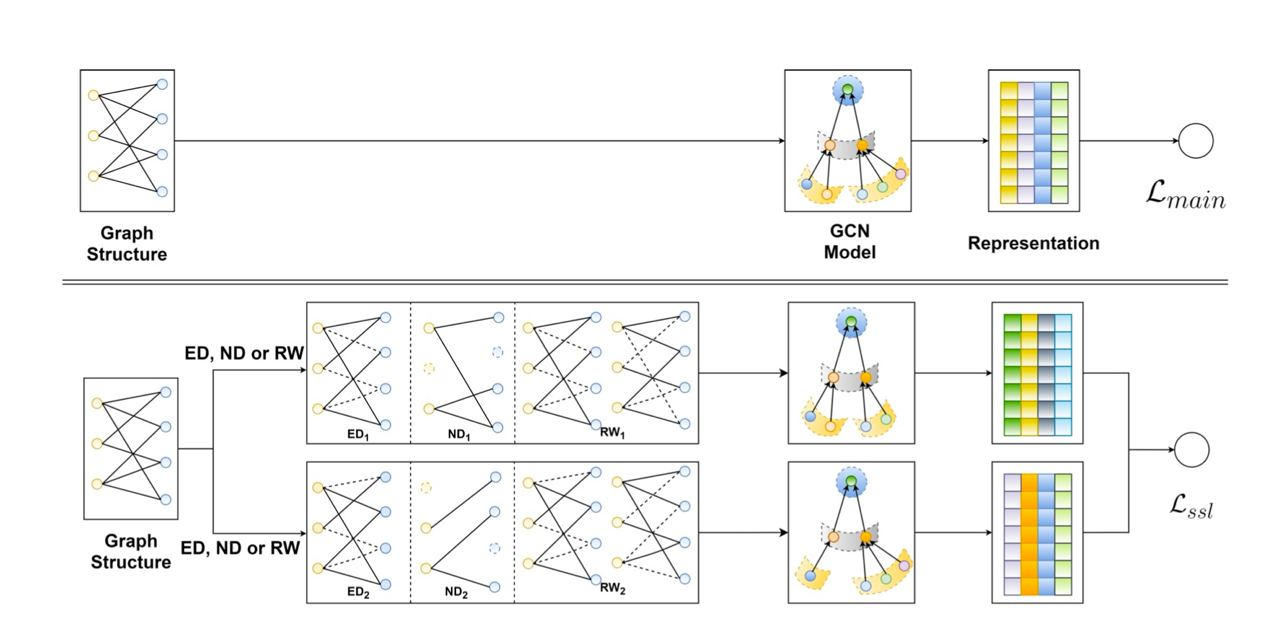
\includegraphics[width=\textwidth]{images/sgl.jpg}
        }
    };
     \node[below=0cm of a] (v) {\tiny SGL\tinycite[SIGIR2021]{wu2021self-sigir} };
   
\end{tikzpicture}


\framebreak

        
    \item Contrastive Loss
        \begin{itemize}
            \item Augmented views of the same user node are treated as the positive pairs (i.e., $\{(z_u^{\prime}, z_u^{\prime \prime})\}$), and the views of different user nodes are treated as the negative pairs (i.e., $\{(z_u^{\prime}, z_v^{\prime \prime}\}$)). 
            \item InfoNCE Loss: Maximization principle  (\textbf{InfoMax}) that aims to \textit{maximize} the correspondence between the representations of the nodes in its different augmented graphs.

\begin{equation*}
\label{eq:info_nce}
\mathcal{L}^{\mathcal{U}}_{\text{NCE}}=\sum_{u \in \mathcal{U}}-\log \frac{\exp \left(sim\left(\mathbf{z}_{u}^{\prime}, \mathbf{z}_{u}^{\prime \prime}\right) / \tau\right)}{\sum_{v \in \mathcal{U}} \exp \left(sim\left(\mathbf{z}_{u}^{\prime}, \mathbf{z}_{v}^{\prime \prime}\right) / \tau\right)}, 
\end{equation*}
where $\tau$ is the temperature hyper-parameters and $sim$ is the similarity function (e.g., cosine function).
            
            \item Analogously, contrastive loss is also adopted on the item side (i.e., $\mathcal{L}^{\mathcal{I}}_{\text{NCE}}$).
The final contrastive loss is the combination of two losses as $\mathcal{L}_{\text{NCE}} = \mathcal{L}^{\mathcal{U}}_{\text{NCE}} + \mathcal{L}^{\mathcal{I}}_{\text{NCE}} $.
        \end{itemize}
\framebreak
    
    \item Joint training scheme $\mathcal{L} = \mathcal{L}_{\text{Rec}} + \lambda_1 \mathcal{L}_{\text{NCE}} + \lambda_2 \mathcal{L}_{\text{Reg}}$
    \begin{itemize}
        \item Contrastive learning in recommender systems usually adopts the joint learning strategy to train their model instead of pre-training and fine-tuning strategies.
        \item Both pretext tasks and downstream tasks are optimized jointly.
        \item  SGL~\tinycite[SIGIR2021]{wu2021self-sigir} demonstrate that joint training will achieve better performance, the pretext tasks and downstream tasks are mutually enhanced with each other.
    \end{itemize}
    
\begin{tikzpicture}[remember picture,overlay]
    \node[anchor=center] (a) at ($(current page.center) + (0.0\textwidth, -0.2\linewidth)$)
    {   
        \resizebox{0.8\textwidth}{!}{
        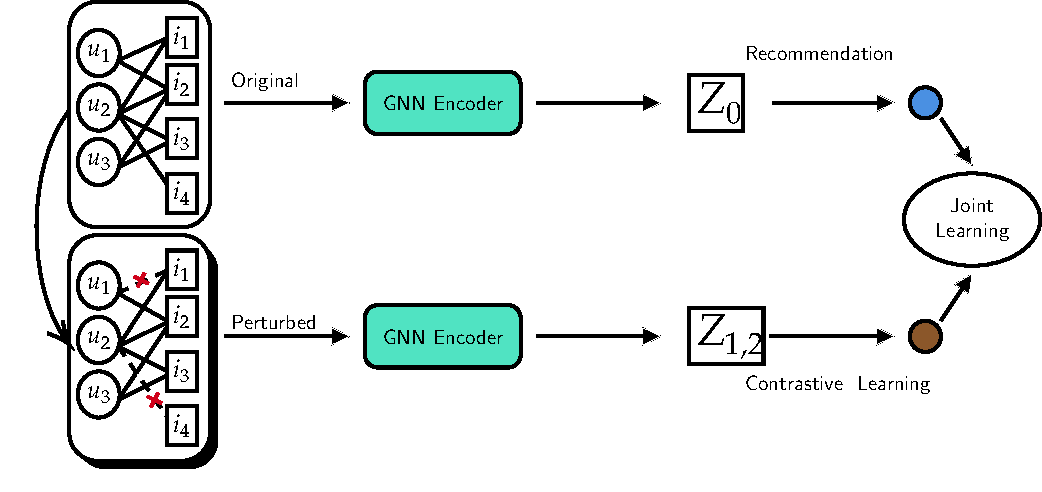
\includegraphics[width=\textwidth]{images/joint_leanring.pdf}
        }
    };
\end{tikzpicture}
           
       

           

\end{itemize}

\end{frame}



\section{Methodology}
\label{sec:model}

\subsection{Framework}

\subsection{Graph Data Augmentation With Edge Operating}
\label{sec:data-aug}

\begin{frame}[allowframebreaks]{Graph Data Augmentation With Edge Operating}
\setlistsep{2ex}{2ex}{0ex}
\begin{itemize}
    \item Edge-Dropping Data Augmentations
    \begin{itemize}
        \item Generally edge-dropping is as follows:
\begin{equation*}
s_{1}(G) = \mathbf{A}_1 = \mathbf{A} \odot \mathbf{M}_1, \quad s_{2}(G) = \mathbf{A}_2 = \mathbf{A} \odot \mathbf{M}_{2},
\end{equation*}
where $\odot$ is the Hadamard product and $\mathbf{M}_1, \mathbf{M}_2 \in \{0, 1\}^{|V| \times |V|}$ are two masking matrices to be applied on the original graph $G$ to generate two augmented graph adjacency matrix $\mathbf{A}_1$ and $\mathbf{A}_2$.
        \item Sampling edges follow a uniform distribution to keep $(1-\rho)\times |\mathcal{E}|$ edges, where $\rho$ is the edge-dropping ratio. $\rho$ is usually set to a small value (e.g., 0.1).
        \item Weakness:
        \begin{itemize}
            \item High complexity of randomly sampling edges from $\mathbf{A}$ is $\mathcal{O}((|V|)^2)$.
            \item Introduce noises by randomly adding edges.
        \end{itemize}
    \end{itemize}

\framebreak

    \item Edge-Operating Data Augmentation
    \begin{itemize}
        \item A new data augmentation in recommender systems (i.e., \textbf{edge-operating} including both edge-adding and edge-dropping).
        \begin{itemize}
            \item Edge Suggestion
            \item Edge Adding
            \item Edge Dropping
        \end{itemize}
    \end{itemize}
\vspace{2em}

 \begin{tikzpicture}[remember picture,overlay]
    \node[anchor=center] (a) at ($(current page.center) + (1cm, -1.5cm)$)
    {
            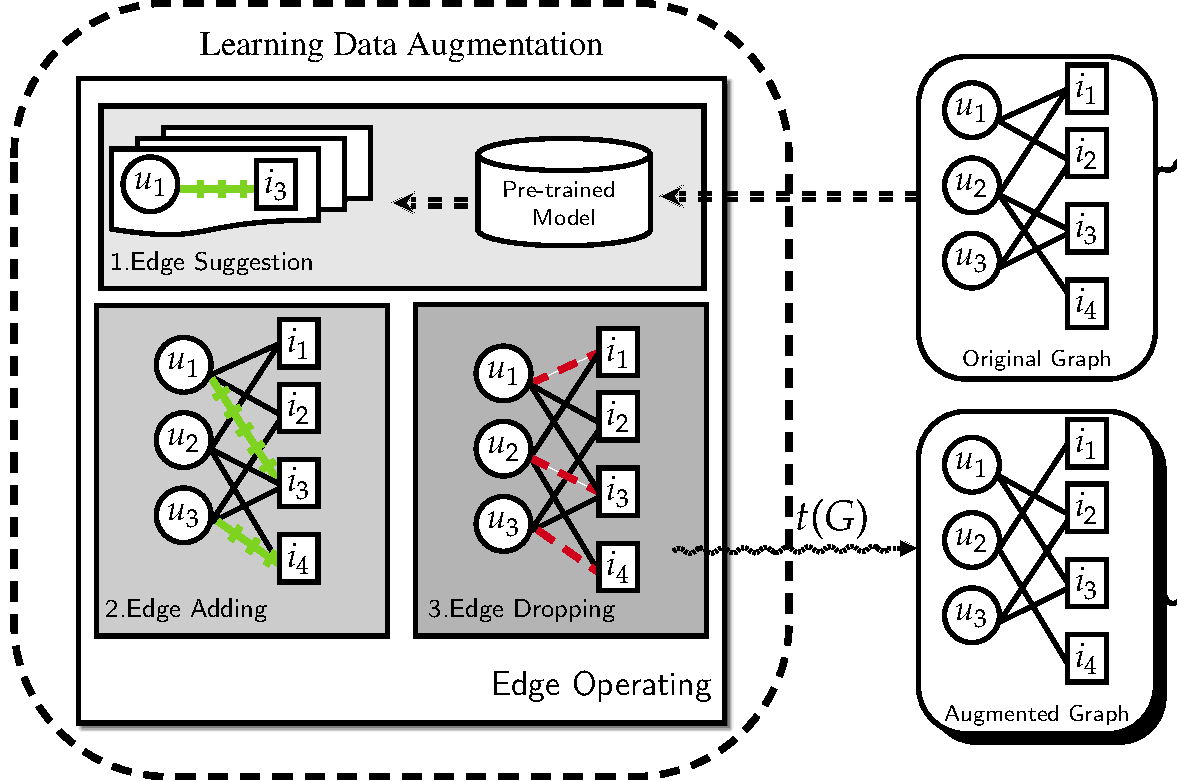
\includegraphics[width=0.6\linewidth]{./images/LDA.pdf}
    };
    \node[anchor=center] (a) at ($(current page.center) + (0, -1em)$){};
\end{tikzpicture}

\end{itemize}
\end{frame}




% % 正如前文提到的,常见的数据增强的方式主要是在丢边
\subsection{Learning Data Augmentation}

\begin{frame}{Learning Data Augmentation}
\begin{itemize}
    \item Learnable edge operator model $t$ 
    \begin{itemize}
        \item We use a Multi-layer Perception (MLP) to learn the weight for every edge candidate $e_{u,i}$ as follows:
\begin{equation*}
    \omega_{u,i}=\operatorname{MLP}\left(\left[z_{u} \odot z_{i}\right] \|  \mathds{1}_{\mathcal{E}}(e_{u,i}) \right),
\end{equation*}
where $\odot$ is the Hadamard product, $z_u$ and $z_i$ are the embeddings for user $u$ and item $i$, $\|$ is the concatenation operator and $\mathds{1}_{\mathcal{E}}(e_{u,i})$ indicates if edge $e_{u,i}$ belongs to original or added edges.
        \item Gumbel-Max reparameterization~\tinycite[ICRL2017]{JangGP17} to get the probability $p_{u,i}$ for edge $e_{u,i}$ by
\begin{equation*}
    \label{eq:p_ui}
    p_{u,i} = \mathrm{sigmoid}(\frac{(\log\delta - \log(1-\delta) + \omega_{u,i})}{\tau}),
\end{equation*}
where $\delta \sim$ Uniform(0,1) and $\tau$ is the temperature hyperparameter. 
        \item We use $p_{u,i}$ to construct augmented graphs
$
t(G)= \mathbf{A}^{\prime} = \left(\begin{array}{cc} \mathbf{0} & \mathbf{P} \\ \mathbf{P}^{\top} & \mathbf{0}\end{array}\right),
$
where $\mathbf{P}\in R^{|\mathcal{U}|\times |\mathcal{I}|}$ is the probability matrix.
        
    \end{itemize}
\end{itemize}

\end{frame}


\subsection{Objective Function} 
\label{sec:loss_function}

\begin{frame}[allowframebreaks]{Objective Function}
\begin{itemize}
    \item InfoMin and InfoMax:
    \begin{itemize}
        \item Overall Objective Functions:
        \begin{equation*}
\label{eq:loss_function}
\begin{aligned}
\min_{t}\  \lambda_t I(f(G); f(t(G)))  + \mathcal{L}(f(t(G)), y) \\
\max_{f}\  I(f(G); f(t(G))) - \mathcal{L}(f(G), y),
\end{aligned}
\end{equation*}
where $I(X_1; X_2)$ is the mutual information between two random variables $X_1$ and $X_2$, $t$ is the data augmentation learner, $f$ is the GNN encoder and $\mathcal{L}$ is the task relevant supervised loss function.
$\lambda_t$ is used to control the influence of $I$ for $t$.
\item $t$: MLP 
\item $f$: LightGCN
\item $\mathcal{L}$: BPR 
\item $I$: InfoNCE Estimator
    \end{itemize}

\begin{tikzpicture}[remember picture,overlay]
    \node[anchor=center] (a) at ($(current page.center) + (2cm, -2.5cm)$)
    {
            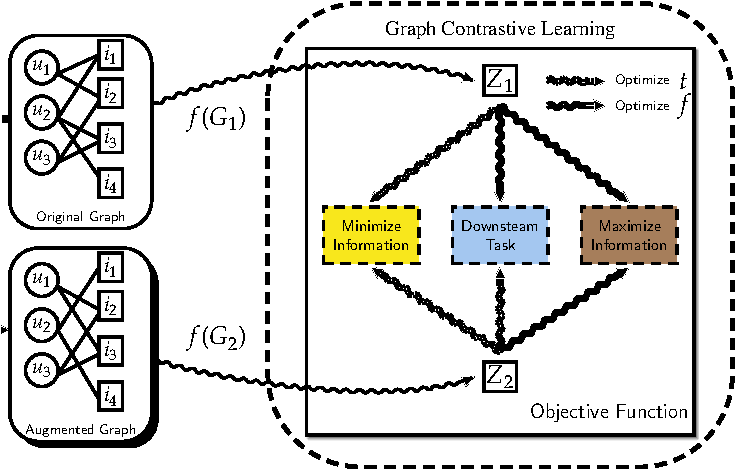
\includegraphics[width=0.4\linewidth]{./images/GCL.pdf}
    };
    \node[anchor=center] (a) at ($(current page.center) + (0, -1em)$){};
\end{tikzpicture}


    
\framebreak

    \item  Mutual Information (MI) Estimator:
    \begin{itemize}
        \item We use InfoNCE as the MI Estimator
        \begin{small}
\begin{equation*}
    I(f(G), f(t(G)) \rightarrow -\mathcal{L}_{\text{NCE}}=\frac{1}{B} \sum_{i=1}^{B} \log \frac{\exp \left(sim\left(z_{i, 1}, z_{i, 2}\right)\right)}{\sum_{i^{\prime}=1, i^{\prime} \neq i}^{B} \exp \left(sim\left(z_{i, 1}, z_{i^{\prime}, 2}\right)\right)},
\end{equation*}
where $sim$ is the cosine similarity to measure the agreement between two representations, $z$ is the node representaton encoded by $f(G)$ and $f(t(G))$, and $B$ is the batch size.
\end{small}
    \end{itemize}
\framebreak
    \item Training LDA-GCL
    \begin{itemize}
        \item Fix $t$:
\begin{equation*}
    \label{eq:fix_t}
   \mathcal{L}_{f} =\mathcal{L}_{\text{BPR}}(f(G), y) +  \lambda_{ssl}\mathcal{L}_{\text{NCE}}\ (f(G), f(t(G))) +  \lambda_{reg} \|f\|^2_{2},
\end{equation*}
where $\lambda_{ssl}$ and $\lambda_{reg}$ are the hyper-parameters to control the weights of the InfoNCE loss function and the regularization term.
        \item Fix  $f$:
\begin{equation*}
   \label{eq:fix_f}
   \mathcal{L}_{t} = \mathcal{L}_{\text{BPR}}(f(t(G)), y) -\lambda_2\mathcal{L}_{\text{NCE}}\ (f(G), f(t(G))) + \lambda_{reg} \|t\|^2_{2},
\end{equation*}
where $\lambda_2 = \lambda_t \times \lambda_{ssl}$ and $\lambda_{reg}$ are the hyper-parameters to control the weights of the InfoNCE loss function and the regularization term.
    \end{itemize}
\end{itemize}

\end{frame}

\subsection{Training LDA-GCL}

\begin{frame}{Training LDA-GCL}
\begin{center}
  \resizebox{!}{0.4\textheight}{
\begin{algorithm}[H]
  \caption{LDA-GCL~ Training Algorithm}
  \label{alg:algorithm1}
  \begin{algorithmic}[1]
    \renewcommand{\algorithmicrequire}{\textbf{Input:}}
    \renewcommand{\algorithmicensure}{\textbf{Output:}}
    \REQUIRE {
      Original bipartite graph $G(\mathcal{U},\mathcal{I}, \mathcal{E})$; 
      Pre-trained GNN encoder $f_0$;
      GNN encoder $f$;
      Edge operator model $t$;
      Epoch $T$;
    }
    
    \ENSURE{
      Node representation $Z$
    }
    \\
    
    \STATE{Generate added edges $\mathcal{E}_1$ from pre-trained model $f_0$.}
    \STATE{Merge added edges $\mathcal{E}_1$ and original edges $\mathcal{E}$ into edge candidates $\mathcal{E}_2$.}
    \STATE{Initialize the parameters of edge operator model $t$ and GNN encoder $f$}

    % \STATE{Initialize original user embeddings $z^0_u$ and item embeddings $z^0_i$, $\forall u \in \mathcal{U}$, $\forall i \in \mathcal{I}$.}
    \FOR{$epoch=1,...,T$}
    \FOR{each mini-batch interactions $B=\{(u_1, i_1, i_2)\}$}
    \STATE{Get node set $V$ with user set $U$ and item set $I$ in mini-batch data}
    
    \tcc{ Optimize $t$}
    
    \STATE{Freeze GNN encoder $f$; unfreeze edge operator $t$}
    \STATE{Apply $t$ on $\mathcal{E}_2$ to get augmented graph $t(G)$ and Apply $f$ to get the embeddings $Z_1, Z_2$ for node $V$ from $G$}
    \STATE{Compute loss in \equref{eq:fix_f} with $Z_1$ and $Z_2$; Back propagation, update $t$.}
    
    \tcc{Optimize $f$}
    \STATE{Freeze edge operator $t$; unfreeze of GNN encoder $f$ }
    \STATE{Apply $t$ on $\mathcal{E}_2$ to get augmented graph $t(G)$ and Apply $f$ to get the embeddings $Z_1, Z_2$ for node $V$ from $G$}
    \STATE{Compute loss in \equref{eq:fix_t} with $Z_1$ and $Z_2$; Back propagation, update $f$.}

    \tcc{Judge early stopping condition}
    \IF{$Z_1$ match the early stopping condition}
    \STATE{Stop training algorithm; Return the best GNN encoder $f_{opt}$}
    \ENDIF
    \ENDFOR
    \ENDFOR
    \RETURN {$Z = f_{opt}(G)$}
  \end{algorithmic}
\end{algorithm}
}
  
\end{center}
\small

\end{frame}


\section{Experiments}
\begin{frame}[c]{RQs}
\begin{itemize}
    \item \textbf{RQ1}: How does LDA-GCL~ perform in recommendation tasks as compared with the state-of-the-art CF models and GCL models?
    \item \textbf{RQ2}: If LDA-GCL~ performs well, what component benefits our LDA-GCL~ in collaborative filtering tasks?     
    \item \textbf{RQ3}: What hyper-parameters affect the effectiveness of the proposed LDA-GCL? 
\end{itemize}
\end{frame}

\subsection{Experimental Settings}

\begin{frame}{Experimental Settings}

\begin{table}[H]
\centering
\caption{Statistics of the datasets used in this paper.}
\label{tb:dataset}
\resizebox{0.6\textwidth}{!}{
\begin{tabular}{c *{4}{r}}
    \toprule
    \textbf{Datasets} & \textbf{\#Users} & \textbf{\#Items} & \textbf{\#Interactions} & \textbf{\%Density}\\
    \midrule
    Yelp 			& 45,478 & 30,709 & 1,777,765 & 0.127 \\
    Gowalla         & 29,859 & 40,989 & 1,027,464 & 0.084 \\
    Amazon-Book 	& 58,145 & 58,052 & 2,517,437 & 0.075 \\
    Alibaba-iFashion & 300,000 & 81,614 & 1,607,813 & 0.007  \\
    \bottomrule
\end{tabular}
}
\end{table}

\begin{itemize}
    \item Datasets: Yelp, Gowalla, Amazon-Book and Alibaba-iFashion.
    \item Data splits: 80/10/10 - training/validation/testing data split 5 times
    \item Baselines: 
    \begin{itemize}
        \item Matrix Factorization: \textbf{BPRMF}/\textbf{NeuMF}/\textbf{DMF}
        \item Graph Neural Networks: \textbf{NGCF}/\textbf{DGCF}/ \textbf{LightGCN}
        \item Graph Contrastive Learning: \textbf{SGL}/\textbf{SimGCL}/\textbf{NCL}
    \end{itemize}
    \item Metrics: Recall@$N$ and NDCG@$N$ (10, 20, 50)
\end{itemize}
\end{frame}

% 
\subsection{Performance Comparision (RQ1)}

\begin{frame}{Performance Comparision}


\begin{table}

% \begin{threeparttable}
\centering
\caption{Performance Comparison of Different Baseline Models. The best result is \textbf{bolded} and the second result is \underline{underlined}. $^*$ indicates the statistical significance for $p<$ 0.05}
\label{tab:exp-main}
\resizebox{0.8\textwidth}{!}{
\begin{tabular}{@{}c|c|ccc|ccc|cccc}
\toprule
 & &\multicolumn{3}{|c|}{Matrix Factorization} & \multicolumn{3}{|c|}{Graph Neural Networks} & \multicolumn{4}{|c}{Graph Contrastive Learning}\\
\midrule
Dataset  & Metric & BPRMF & NeuMF & DMF  & NGCF & DGCF & LightGCN & SGL & SimGCL & NCL & LDA-GCL~ \\ 

\midrule



\multirow{6}{*}{Yelp} 
& Recall@10 & 0.0499 & 0.0367 & 0.0372 & 0.0514 & 0.0606 & 0.0616 & 0.0664  & \underline{0.0743} & 0.0713 &\textbf{0.0751}$^*$ \\ 
& Recall@20 & 0.0829 & 0.0629 & 0.0631 & 0.0857 & 0.0987 & 0.1001 & 0.1072  & \underline{0.1185} & 0.1135 & \textbf{0.1190}$^*$  \\ 
& Recall@50 & 0.1549 & 0.1227 & 0.1215 & 0.1596 & 0.1798 & 0.1817 & 0.1928  & \underline{0.2068} & 0.1997 & \textbf{0.2101}$^*$  \\
& NDCG@10 & 0.0335 & 0.0242 & 0.0248 & 0.0346 & 0.0412 & 0.0419 & 0.0456  & \underline{0.0515} & 0.0489 & \textbf{0.0518}$^*$ \\
& NDCG@20 & 0.0438 & 0.0324 & 0.0327 & 0.0453 & 0.0530 & 0.0538 & 0.0581 &  \underline{0.0652}  & 0.0619 & \textbf{0.0653}$^*$  \\
& NDCG@50 & 0.0622 & 0.0477 & 0.0476 & 0.0642 & 0.0738 & 0.0748 & 0.0801  & \underline{0.0878} & 0.0841 &\textbf{0.0886}$^*$ \\
\midrule



\multirow{6}{*}{Amazon-Book} 
& Recall@10 & 0.0619 & 0.0442 & 0.0313 & 0.0575 & 0.0787 & 0.0783 & 0.0844 & 0.0872 &\underline{0.0947} & \textbf{0.0975}$^*$ \\
& Recall@20 & 0.0971 & 0.0726 & 0.0522 & 0.0920 & 0.1191 & 0.1210 & 0.1281 & 0.1251 & \underline{0.1395} & \textbf{0.1456}$^*$  \\
& Recall@50 & 0.1676 & 0.1331 & 0.0984 & 0.1624 & 0.1965 & 0.2055 & 0.2117 & 0.1934 & \underline{0.2201} & \textbf{0.2346}$^*$ \\
& NDCG@10 & 0.0431 & 0.0295 & 0.0216 & 0.0400 & 0.0563 & 0.0553 & 0.0606 & 0.0643 & \underline{0.0685} & \textbf{0.0699}$^*$\\
& NDCG@20 & 0.0537 & 0.0382 & 0.0280 & 0.0505 & 0.0681 & 0.0682 & 0.0739 & 0.0758 & \underline{0.0822} & \textbf{0.0845}$^*$  \\
& NDCG@50 & 0.0721 & 0.0539 & 0.0400 & 0.0688 & 0.0887 & 0.0902 & 0.0956 & 0.0936 &\underline{0.1034} & \textbf{0.1078}$^*$\\
 \midrule
 


\multirow{6}{*}{Gowalla} 
& Recall@10 & 0.1040 & 0.0882 & 0.0634 & 0.0992 & 0.1343 & 0.1355 & 0.1386 & 0.1487  & \underline{0.1496} & \textbf{0.1505} \\
& Recall@20 & 0.1525 & 0.1307 & 0.0945 & 0.1462 & 0.1917 & 0.1969 & 0.1969 & 0.2123 & \underline{0.2131} & \textbf{0.2144}  \\
& Recall@50 & 0.2476 & 0.2161 & 0.1559 & 0.2383 & 0.2972 & 0.3093 & 0.3055 & 0.3208 & \underline{0.3228} & \textbf{0.3284}$^*$  \\
& NDCG@10 & 0.0738 & 0.0603 & 0.0450 & 0.0703 & 0.0963 & 0.0961 & 0.0999 & 0.1078 & \underline{0.1081} & \textbf{0.1085}  \\
& NDCG@20 & 0.0878 & 0.0727 & 0.0540 & 0.0838 & 0.1127 & 0.1136 & 0.1166 & 0.1259 & \underline{0.1263} & \textbf{0.1268}  \\
& NDCG@50 & 0.1109 & 0.0935 & 0.0692 & 0.1062 & 0.1384 & 0.1411 & 0.1431 & 0.1525 & \underline{0.1534} & \textbf{0.1547}  \\
\midrule



\multirow{6}{*}{Alibaba-iFashion} 
& Recall@10 & 0.0297 & 0.0157 & 0.0138 & 0.0355 & 0.0361 & 0.0402 & \underline{0.0518} & 0.0450 & 0.0490 & \textbf{0.0605}$^*$ \\
& Recall@20 & 0.0458 & 0.0264 & 0.0229 & 0.0565 & 0.0549 & 0.0612 & \underline{0.0774} & 0.0651 & 0.0729 & \textbf{0.0882}$^*$ \\
& Recall@50 & 0.0784 & 0.0501 & 0.0443 & 0.0994 & 0.0910 & 0.1015 & \underline{0.1258} & 0.1029 & 0.1178 & \textbf{0.1381}$^*$ \\
& NDCG@10 & 0.0158 & 0.0079 & 0.0071 & 0.0185 & 0.0194 & 0.0216 & \underline{0.0280} & 0.0252 & 0.0267 & \textbf{0.0335}$^*$  \\
& NDCG@20 & 0.0199 & 0.0106 & 0.0094 & 0.0237 & 0.0241 & 0.0269 & \underline{0.0344} & 0.0303 & 0.0328 & \textbf{0.0405}$^*$ \\
& NDCG@50 & 0.0264 & 0.0152 & 0.0137 & 0.0323 & 0.0313 & 0.0350 & \underline{0.0440} & 0.0378 & 0.0417 & \textbf{0.0504}$^*$  \\

\bottomrule
\end{tabular}
}

% \begin{tablenotes}
%       \item The best result is \textbf{bolded} and the second result is \underline{underlined}. $^*$ indicates the statistical significance for $p<$ 0.05.
% \end{tablenotes}
% \end{threeparttable}
\end{table}
\end{frame}




\subsection{Benefits of LDA-GCL~ (RQ2)}
\label{sec:add_graph}

\begin{frame}{Sparsity Analysis}
\begin{figure}[!t]
  \centering

\subfloat[Gowalla\label{fig:group-analysis-1}]{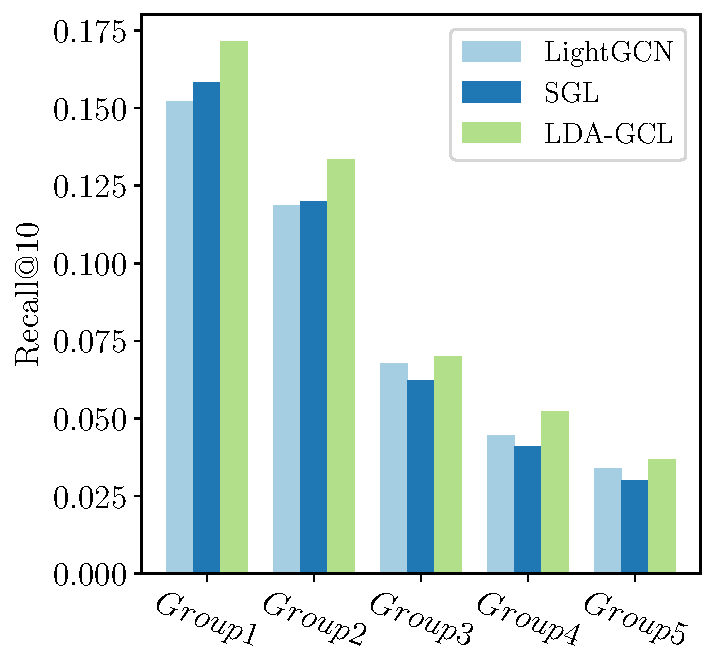
\includegraphics[width=0.45\textwidth]{images/gowalla-groups.pdf}}\qquad
  \subfloat[Alibaba-iFashion\label{fig:group-analysis-2}]{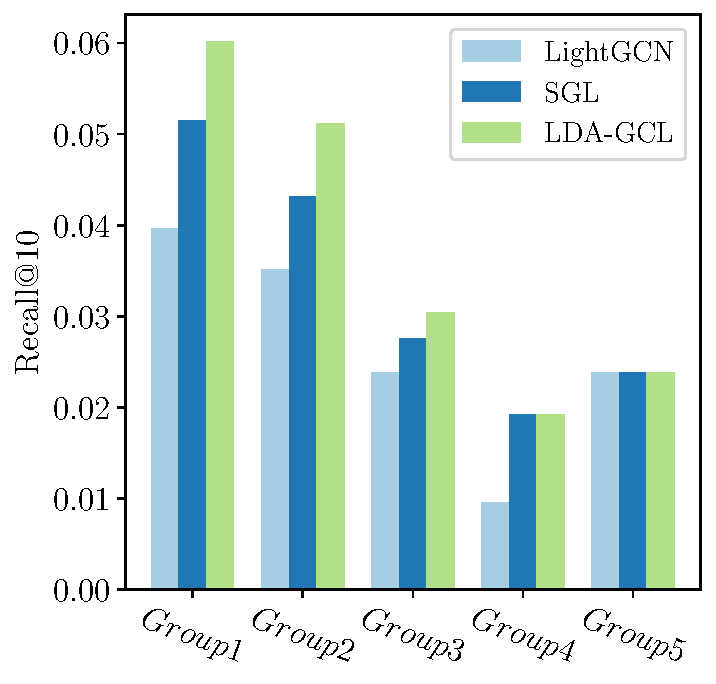
\includegraphics[width=0.45\textwidth]{images/alibaba-groups.pdf}}

  \caption{Performance analysis over different users groups.
  $G_1$ is the group of users with the \textit{lowest} interaction number.}
  \label{fig:group-analysis}
\end{figure}
 
\end{frame}

\begin{frame}{Ablation Study}

 
\begin{table}
\vspace{-1em}
\centering
\caption{Performance comparison of different variants of LDA-GCL.}
\label{tab:ablation}
\resizebox{0.85\textwidth}{!}{
\begin{tabular}{c|cc|cc}
\toprule
\multicolumn{1}{c}{\multirow{2}{*}{Method}} & \multicolumn{2}{c}{Gowalla}                            & \multicolumn{2}{c}{Alibaba-iFashion}                                    \\
\multicolumn{1}{c}{}                        & \multicolumn{1}{c}{Recall@10} & \multicolumn{1}{c}{NDCG@10} & \multicolumn{1}{c}{Recall@10} & \multicolumn{1}{c}{NDCG@10} \\ \midrule
LightGCN & 0.1342	& 0.0962 & 0.0395	& 0.0212 \\
\midrule
DA-GCL(0.0,0.0) & 0.1488 & 0.1085 & 0.0497 & 0.0274 \\
DA-GCL(0.1,0.0) & 0.1492 & 0.1083 & 0.0529 & 0.0289 \\
DA-GCL(0.0,0.1) & 0.1487 & 0.1067 & 0.0544 & 0.0299 \\
DA-GCL(0.1,0.1) & 0.1479 & 0.1063 & 0.0553 & 0.0303 \\
DA-GCL(0.0,0.5) & 0.1412 & 0.1010 & 0.0533 & 0.0290 \\
DA-GCL(0.1,0.5) & 0.1409 & 0.1003 & 0.0542 & 0.0296 \\
DA-GCL(0.0,1.0) & 0.1369 & 0.0973 & 0.0520 & 0.0282 \\
DA-GCL(0.1,1.0) & 0.1359 & 0.0963 & 0.0526 & 0.0285 \\
\midrule
LDA-GCL (w NGCF) & 0.1488 & 0.1078 & 0.0589 & 0.0322 \\
LDA-GCL (w/o EA) & 0.1499 & 0.1087 & 0.0579 & 0.0319 \\
LDA-GCL & 0.1512 & 0.1090 & 0.0599 & 0.0330 \\
\bottomrule
\end{tabular}
}
\end{table}
\end{frame}




\subsection{Parameter Analysis (RQ3)}

\section{Conclusion and Future Work}
\label{sec:conclusion}
\begin{frame}{Conclusion and Future Work}

\begin{itemize}
    \item Conclusion
    \begin{itemize}
        \item A theoretically motivated learnable data augmentation model for GCL in recommendation, instead of  heuristic designs. (\textbf{InfoMin} and \textbf{InfoMax})
        \item An adversarial framework that can better enhance the effect of GCL in the recommendation.
        \item Our model achieves state-of-the-art performance on several public benchmark datasets.
        \item The relevant analytical experiments prove the efficiency of the model design.
    \end{itemize}
    \item Future work
    \begin{itemize}
        \item To make improvements on the efficiency in future work.
A potential boosting scheme is the pre-trained edge operator models.
    \end{itemize}
\end{itemize}
\end{frame}


\qapage

\refpage


\end{document}

